\chapter{Genetic Code as Distinction Algebra}

\section{The Genetic Code}

64 codons map to 20 amino acids + stop signals.

This is not arbitrary. DD reveals the structure.

\section{Why Triplets?}

\subsection{The Minimal Encoding Problem}

4 bases. 20 amino acids to encode.

\begin{align}
4^1 &= 4 \quad \text{(insufficient)} \\
4^2 &= 16 \quad \text{(insufficient)} \\
4^3 &= 64 \quad \text{(sufficient with redundancy)}
\end{align}

\subsection{DD Interpretation}

Triplet = \textbf{triad} at genetic level.

\begin{center}
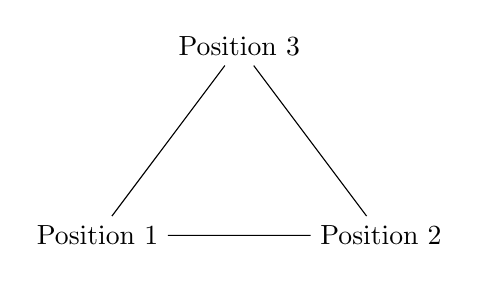
\begin{tikzpicture}[scale=1.2]
\node (a) at (0,0) {Position 1};
\node (b) at (3,0) {Position 2};
\node (c) at (1.5,2) {Position 3};
\draw (a) -- (b) -- (c) -- (a);
\end{tikzpicture}
\end{center}

Three positions = minimal closure for biological information.

\subsection{Why Not Quadruplets?}

$4^4 = 256$. Too much redundancy. Wasteful.

Evolution found the \emph{minimal} triadic encoding.

\section{The Redundancy Structure}

\subsection{Wobble Position}

Third codon position is most variable. Often doesn't affect amino acid.

\begin{center}
\begin{tabular}{c|c}
\textbf{Codon} & \textbf{Amino Acid} \\
\hline
GCU & Ala \\
GCC & Ala \\
GCA & Ala \\
GCG & Ala \\
\end{tabular}
\end{center}

\subsection{DD Interpretation}

Position 1-2: Core distinction (which amino acid class)

Position 3: Fine-tuning (redundancy, error tolerance)

The triad has hierarchy: not all positions equal.

\section{Amino Acid Properties}

\subsection{The Property Space}

20 amino acids span a property space:
\begin{itemize}
\item Hydrophobicity (water-hating vs water-loving)
\item Charge (positive, negative, neutral)
\item Size (small, medium, large)
\item Special features (aromatic, sulfur, etc.)
\end{itemize}

\subsection{Why These Properties?}

These are the \emph{distinctions that matter} for protein function:
\begin{itemize}
\item Hydrophobicity: Inside vs outside of protein
\item Charge: Binding interactions
\item Size: Fitting into active sites
\item Special: Catalysis, cross-linking
\end{itemize}

\subsection{The 20 as Basis}

20 amino acids = basis vectors in biochemical distinction space.

Any protein function can be constructed from combinations of these 20 distinctions.

\section{Codon Assignment}

\subsection{Is It Random?}

No. Similar codons encode similar amino acids.

Example: All GCN codons $\to$ Alanine (small, hydrophobic)

\subsection{Error Minimization}

The code minimizes effect of mutations:
\begin{itemize}
\item Single-base changes usually give similar amino acid
\item Worst mutations (changing all properties) are rare
\end{itemize}

This is \emph{error-correcting code} evolved over billions of years.

\subsection{DD Structure}

The genetic code is a \textbf{morphism} in distinction space:

\[
\phi: \text{Codon Space} \to \text{Amino Acid Space}
\]

such that:
\[
d(\text{codon}_1, \text{codon}_2) \text{ small} \Rightarrow d(\text{aa}_1, \text{aa}_2) \text{ small}
\]

Distinctions are preserved under mapping.

\section{The Start and Stop}

\subsection{Start Codon}

AUG = Methionine = Start

Every protein begins with the same distinction: ``here begins''.

\subsection{Stop Codons}

UAA, UAG, UGA = Stop

Three stop codons. Why three?

DD: Termination is \emph{triadic closure}. Three ways to close the reading frame.

\section{Universality}

\subsection{One Code for All Life}

Nearly all life uses the same genetic code.

This suggests:
\begin{enumerate}
\item Common ancestor (historical contingency)
\item \textbf{OR} Optimal solution (necessity)
\end{enumerate}

\subsection{DD Argument}

The genetic code is not just historical accident. It's a \emph{local optimum} in the space of possible codes.

Other codes exist (slight variations in mitochondria, some organisms), but the standard code dominates because it's near-optimal for error minimization.

\section{Information Density}

\subsection{Bits per Codon}

\begin{align}
\text{Codon entropy} &= \log_2(64) = 6 \text{ bits} \\
\text{Amino acid entropy} &= \log_2(20) \approx 4.3 \text{ bits} \\
\text{Redundancy} &\approx 1.7 \text{ bits/codon}
\end{align}

\subsection{Why Not Maximum Density?}

Maximum density would be no redundancy: 20 codons for 20 amino acids.

But this has no error tolerance. The 1.7 bits of redundancy are \emph{invested} in robustness.

DD: Optimal information systems balance \emph{distinction capacity} with \emph{distinction stability}.

\section{The Code as Algebra}

\subsection{Algebraic Structure}

Codons form a group under certain operations:
\begin{itemize}
\item Complement (A$\leftrightarrow$U, G$\leftrightarrow$C)
\item Reverse
\item Reading frame shifts
\end{itemize}

\subsection{Symmetries}

The code has partial symmetries:
\begin{itemize}
\item Pyrimidine/purine structure
\item Amino/keto structure
\item Position-dependent patterns
\end{itemize}

These symmetries reflect the underlying chemistry but also \emph{distinction algebra}.

\section{Evolution of the Code}

\subsection{Frozen Accident?}

Crick's hypothesis: Code is frozen accident. Once established, too costly to change.

\subsection{DD Alternative}

Code evolved toward optimum. ``Frozen'' not because arbitrary but because \emph{optimal}. No improvement possible without major cost.

The code is frozen because it reached the attractor, not because it got stuck.

\section{Summary}

The genetic code is not arbitrary assignment. It is:

\begin{enumerate}
\item \textbf{Triadic}: Codon triplets reflect universal triad structure
\item \textbf{Error-minimizing}: Distinctions preserved under mutation
\item \textbf{Near-optimal}: Close to best possible code
\item \textbf{Universal}: Same solution found by all life
\end{enumerate}

\begin{center}
\fbox{\parbox{0.8\textwidth}{
The genetic code is distinction algebra written in chemistry.

$\Delta$ (physics) $\to$ codon (genetics) $\to$ protein (function)

One principle at all levels.
}}
\end{center}
